%%%%%%%%%%%%%%%%%%%%%%%%%%%%%%%%%%%%%%%%%%%%%%%%%%

% Latex Kapitel erstellen. 
% 		Kopiere 'texPandoc/*.tex' nach 'content/tex' 
% 		'content/tex' **Handarbeit... für opt. Ergebnisse!** 
% 		Kopiere 'archiv/inhalt.tex' nach 'content/' 
% 		make -- Latex-PDF erstellen 
% ju 16-Dez-2022 inhalt.tex

%%%%%%%%%%%%%%%%%%%%%%%%%%%%%%%%%%%%%%%%%%%%%%%%%%

% content/

\chapter{01-Grundlagen-Elektrotechnik}
%\input{content/tex/01-Grundlagen-Elektrotechnik}
\chapter{02-Grundlagen-Elektrotechnik2}
%\input{content/tex/02-Grundlagen-Elektrotechnik2}
\chapter{02-Sensoren-und-Aktoren}
%\input{content/tex/02-Sensoren-und-Aktoren}
\chapter{03-Hochvolt}
%\input{content/tex/03-Hochvolt}
\chapter{04-Generator}
%\input{content/tex/04-Generator}
\chapter{05-Datenbus}
%\input{content/tex/05-Datenbus}
\chapter{Diagnose}
%%ju 31-Dez-22 Diagnose.tex
\textbf{Fehlersuche in einem immer stärker vernetzten Fahrzeugsystem}
(\textcite{respondeck:2019:servicetechniker}).

\begin{enumerate}
\item
  \textbf{Fahrzeugannahme}

  \begin{itemize}
  \item
    Das Fahrzeug sollte im Beisein des Kunden einer \emph{Sicht- und
    Funktionsprüfung} unterzogen werden und den Kunden zu dem Fehler
    befragen.
  \item
    kurzen >>Rundum-Check<< des Fahrzeugs, um weitere
    (sicherheitsrelevante) Mängel aufdecken. In diesem Zusammenhang
    können auch Vorschäden dokumentiert und dem Kunden gezeigt werden,
    um etwaigen Ansprüchen nach Rückgabe des Fahrzeugs entgegenzuwirken.
    Ein Foto von allen Seiten hilft im Streitfall bei der Klärung.
  \item
    Bei \textbf{sporadischen Fehlern} zu hinterfragen, unter welchen
    Umständen und bei welchen Bedingungen der Fehler aufgetreten ist, um
    ihn zu reproduzieren, zu können.

    \begin{itemize}
    \item
      Betriebszustand und Fahrsituation (Motor kalt/warm; Last;
      Drehzahl; Fahrgeschwindigkeit; Beschleunigen/Verzögern;
      Rechts-/Linkskurve usw.)
    \item
      Einsatzbedingungen (hohe/geringe Außentemperatur; Witterung
      Beispiel: Nässe, Regen)
    \item
      Schaltzustände von Teilsystemen (Licht an/aus; Klimaanlage,
      Sitzheizung etc. an/aus)
    \item
      Besonderheiten (Anhängerbetrieb; Zubehör im Innenraum $\to$
      elektromagnetische Störungen/Störung des Bordnetzes durch
      angeschlossene Geräte
    \item
      Technische Änderungen (Motoreingriffe; Umbereifung;
      Fahrwerksänderungen)
    \item
      Kürzlich von einer anderen Werkstatt durchgeführte Reparaturen
    \end{itemize}
  \item
    korrekten \textbf{Fahrzeugschlüssel} vom Kunden übernehmen. (sog.
    Benutzer-Adaption)

    \begin{itemize}
    \item
      Sitz und Spiegeleinstellung, Radiosender und -lautstärke
    \item
      Aktivierung/Deaktivierung von Assistenzsystemen
      (Fahrlichtsteuerung, Regen-/Lichtsensor, Einparkassistent,
      Spurhalteassistent)
    \item
      Tippblinken
    \item
      Automatisches Verriegeln während der Fahrt, automatisches
      Wiederverschließen
    \item
      Ansprechverhalten des Fahrpedals
    \item
      Schaltzeitpunkt des automatischen Getriebes
    \end{itemize}
  \end{itemize}
\item
  \textbf{Fehlerspeicher auslesen}

  \begin{itemize}
  \item
    bei >>Mehreren Kundenbeanstandungen<< im ersten Schritt sollte bei
    der Bewertung der Fehler eine gemeinsame Ursache in Betracht gezogen
    und erst, wenn diese auszuschließen ist, jeder Fehler für sich
    betrachtet werden.
  \item
    gesamten Fehlerspeicher des Fahrzeugs auslesen und bei mehreren
    Fehlern zunächst eine gemeinsame Ursache zu suchen.
  \item
    Vor dem Löschen eines Fehlerspeichers dokumentieren
  \item
    \textbf{Klassische Fehler} vs.~\textbf{Plausibilitätsfehler}
  \end{itemize}
\item
  \textbf{Messwerte/Istwerte/Parameter auslesen}

  \begin{itemize}
  \item
    Prüfen, ob die vom SG mithilfe der Sensorik erfassten Daten der
    Realität entsprechen.
  \item
    Im Zweifel sollten die Werte mithilfe eines separaten Messgerätes
    ermittelt und abgeglichen werden.
  \end{itemize}
\item
  \textbf{Stellgliedtest bei Fehlern im Bereich der Aktorik}

  \begin{itemize}
  \item
    Bauteil mithilfe des Diagnosegeräts ansteuern oder anhand von
    Messwerten überprüfen, ob es reagiert. Prüfen, ob das gewünschte
    Ergebnis tatsächlich erzielt wird.
  \item
    Der Stellgliedtest sollte über das Diagnosegerät durchgeführt
    werden. Eine Überprüfung durch >>Provozieren<< einer Ansteuerung ist
    nicht aussagekräftig, da oftmals nicht alle Bedingungen für das
    Ansteuern des jeweiligen Aktors bekannt sind. Selbst der Vergleich
    mit einem anderen Fahrzeug (gleiches Modell, gleicher Motor,
    gleiches Baujahr) scheitert, wenn sich der Stand der Software der SG
    unterscheidet.
  \end{itemize}
\item
  \textbf{Messungen mit Multimeter und Oszilloskop}

  \begin{itemize}
  \item
    sollte es Hinweise auf fehlerhafte Sensoren, Aktoren oder Systeme
    geben. Ursache des Fehlers ermitteln.
  \item
    Die Größen Spannung, Strom und Widerstand müssen mithilfe der
    Prüfanleitung des Herstellers gemessen werden.
  \end{itemize}
\end{enumerate}

\textbf{Sporadischer Fehler} also wiederkehrend, aber nicht permanent
vorhanden

\textbf{Klassische Fehler} sind solche, bei denen das SG ein Problem des
jeweiligen Bauteils messtechnisch ermittelt und den Fehler (Beispiel:
>>Signalspannung zu hoch<<) als solchen im SG hinterlegt hat. Beim
Auftreten solcher Fehler kann man sofort mit der Fehlersuche im Rahmen
von Messungen im Bereich des jeweiligen Bauteils beginnen.

\textbf{Plausibilitätsfehler} legt das SG dagegen im Fehlerspeicher ab,
wenn die ankommenden Informationen unplausibel sind, also nicht
zueinanderpassen oder Sprünge enthalten, die ohne weitere Informationen
nicht zu erklären sind. Beim Auftreten von Plausibilitätsfehlern sollte
man klären, welche unpassenden Informationen zu dem Fehler geführt
haben.

\textbf{Beispiel 1) Fehler: Heißfilmluftmassenmesser (Diesel) >>Signal
unplausibel<<}

Der Heißfilmluftmassenmesser hat beim Diesel hauptsächlich die Aufgabe,
die Volllastmenge zu begrenzen und die Abgasrückführrate zu ermitteln.

Die AGR-Rate wird bestimmt, indem das SG die Soll-Luftmasse im aktuellen
Betriebszustand aus Hubraum, Drehzahl, Ladedruck usw. ermittelt, und die
vom Luftmassenmesser ermittelte Ist-Luftmasse hiervon abzieht. Bei einer
AGR-Rate von $10~\%$ sollte die vom Luftmassenmesser ermittelte
Luftmasse also $10~\%$ geringer sein, als die theoretisch unter den
aktuellen Bedingungen angesaugte Luftmasse. Wäre nun beispielsweise die
Abgasrückführung verrußt, so reduziert sich die rückgeführte Abgasmenge
bei gleicher Stellung des AGR-Ventils. Der Rückgang der vom
Heißfilmluftmassenmesser ermittelten Luftmasse läge dann unter $10~\%$
und das SG meldet, dass das >>Signal unplausibel<< ist.

\textbf{Beispiel 2) Fehler: Heißfilmluftmassenmesser (Diesel) >>Signal
unplausibel<<}

Der gleiche Fehler des Heißfilmluftmassenmessers kann auftreten, wenn
der Luftfilter erneuert wird, ohne dies dem SG durch das Bestätigen der
jeweiligen Wartung mitzuteilen. Das SG erkennt nach dem Motorstart, dass
sich die Luftmasse unter sonst gleichen Bedingungen gegenüber dem
letzten Fahrzyklus, deutlich erhöht hat. Da es keine Informationen über
einen Luftfilterwechsel erhalten hat, ist dieser >>Sprung<< der
Luftmasse unplausibel. Der Fehler wird im Fehlerspeicher abgelegt.

\textbf{Beispiel 3) Fehler: steigender Kraftstoffverbrauch, Fehler in
AGR-System oder Vorglühanlage}

Ist es am Motortemperaturfühler zu einem Übergangswiderstand gekommen
(Beispiel: durch Korrosion am Steckkontakt), so steigt der ohmsche
Widerstand der Messschaltung. Den erhöhten Widerstand nimmt das SG als
geringere Temperatur auf. Motortemperaturfühler sind in der Regel
NTC-Widerstände $\to$ negativer Temperatur-Koeffizient $\to$
fallender Widerstand bei steigender Temperatur. Solange die ermittelten
Werte innerhalb des plausiblen Bereichs bleiben (Beispiel:
$> -40^\circ\text{C}$), wertet das SG die Information aus. Der Fehler
wird nicht erkannt, zeigt jedoch seine Auswirkungen (Beispiel:
steigender Kraftstoffverbrauch, Fehler in AGR-System oder
Vorglühanlage). Beim Blick in die Messwerte fällt jedoch schnell auf,
dass eine Motortemperatur von $-20^\circ\text{C}$ an einem warmen
Sommertag nicht stimmen kann.

\textbf{Digital} ziffernmäßig, stufenweise, sprungweise

\textbf{Analog} gleichartig, stetig, stufenlos

\textbf{Multimeter}

\begin{itemize}
\item
  Bei Widerstandsmessungen darf das Bauteil nicht unter Spannung stehen.
\item
  Vor dem Ablegen des Messgerätes den Messbereichsschalter in den
  höchsten Wechselspannungsbereich schalten. Dies schützt Gerät und
  Anwender bei unsachgemäßem Einsatz ohne vorherige Einstellungen.
\end{itemize}

\textbf{Oszilloskop} dynamische Messungen (frequente Spannungen oder
eine pulsweitenmodulierte Ansteuerung erfassen, Spannungsverläufe
darstellen). Ermöglicht eine Auswertung des kompletten Arbeitsbereichs
des Sensors.

\begin{itemize}
\item
  Signalspannung des Potenziometers
\item
  Drehzahl- und Bezugsmarkengeber
\item
  Messen des Tastverhältnisses
\item
  Induktionsgeber
\item
  Hallgebersignal
\end{itemize}

\section{Ablauf der Messungen}\label{ablauf-der-messungen}

>>Alle Spannungsmessungen erfolgen unter Last, d.h., es werden keine
Stecker abgezogen.<< Erfolgt die Spannungsmessung bei abgezogenem
Stecker, ist der Stromkreis unterbrochen. Da jetzt kein Strom mehr
fließt, wirken sich Übergangswiderstände nicht mehr aus und die
durchgeführten Messungen sind nicht aussagekräftig.

\textbf{Sensor-Prüfung}

\begin{enumerate}
\item
  \textbf{Erfassen der Signalspannung am SG}

  \begin{itemize}
  \item
    prüfen, ob SG tatsächlich ein fehlerhaftes Signal bekommt, oder ob
    ein fehlerfreies Signal fehlerhaft ausgewertet wird.
  \end{itemize}
\item
  \textbf{Erfassen der Signalspannung am Sensor}

  \begin{itemize}
  \item
    Ist die Signalspannung in Ordnung und am SG fehlerhaft, ist die
    Signalleitung zu überprüfen.
  \item
    Ist die Signalspannung hier fehlerhaft, muss zwischen zwei Fällen
    unterschieden werden:

    \begin{enumerate}
    \def\labelenumii{\arabic{enumii}.}
    \item
      Signalspannung $0~V$: Signalleitung auf Masseschluss prüfen
      ($\to$ Messung 3)
    \item
      Signalspannung $\neq 0~V$ ($\to$ Messung 3)
    \end{enumerate}
  \end{itemize}
\item
  \textbf{Überprüfen der Spannungsversorgung am Sensor}

  \begin{itemize}
  \item
    Sollwert: $5 \pm 0,02~V$ (vgl. Werkstatthandbuch)
  \end{itemize}
\item
  \textbf{Überprüfen der Spannungsversorgung am SG}

  \begin{itemize}
  \item
    Ist die Spannungsversorgung hier in Ordnung und am Sensor gestört,
    sind die Leitungen zum Sensor zu prüfen.
  \item
    Ist die Spannungsversorgung hier gestört, muss geprüft werden, ob
    alle Voraussetzungen gegeben sind, damit das SG eine
    Versorgungsspannung bereitstellt.
  \end{itemize}
\item
  \textbf{Überprüfen der Leitungen}

  \begin{itemize}
  \item
    Spannungsfall über jede elektrische Leitung messen. Hierzu werden
    die beiden Enden der Leitung mit dem Multimeter verbunden und die
    Spannung gemessen. Sie sollte gerade im Bereich der Sensorik nahe
    $0~V$ liegen.
  \item
    Prüfen, ob Leitungen mit einer Plusleitung oder mit Masse verbunden
    sind. Hierzu wird die Leitung aus dem Stromkreis getrennt (alle
    Stecker ab) und anschließend mit dem Multimeter an beiden Enden der
    Leitung jeweils einmal gegen Plus und Masse gemessen. Alle Messungen
    sollten mit dem Ergebnis $0~V$ enden.
  \end{itemize}
\item
  \textbf{Überprüfung des SGs}

  \begin{itemize}
  \item
    SG-Eingänge lassen sich mithilfe einer simulierten Signalspannung
    überprüfen. (Beispiel: geeignete Spannungsquelle oder einer
    Widerstandsdekade)
  \end{itemize}
\end{enumerate}

\textbf{Aktor-Prüfung}

\begin{enumerate}
\item
  \textbf{Überprüfen der Spannungsversorgung am Aktor}

  \begin{itemize}
  \item
    Hierzu muss der jeweilige Aktor eingeschaltet werden. Dies geschieht
    entweder manuell (Beispiel: Licht, Heckscheibenheizung) oder mittels
    Stellgliedtest (Beispiel: AGR-Ventil, Stellmotor-Saugrohr). Da viele
    Aktoren aktuell pulsweitenmoduliert angesteuert werden, empfiehlt
    sich das Oszilloskop. Die gemessene Spannung liegt i.d.R. bei
    Bordnetzspannung.
  \item
    Ist die Versorgungsspannung in Ordnung, der Aktor reagiert jedoch
    nicht, kann von einem Defekt des Aktors ausgegangen werden.
  \item
    Ist die gemessene Spannung nicht in Ordnung ($\to$ Messung 2).
  \end{itemize}
\item
  \textbf{Überprüfen der Spannungsversorgung am SG}

  \begin{itemize}
  \item
    Ist die Spannungsversorgung hier in Ordnung und am Sensor gestört,
    sind die Leitungen zum Sensor zu prüfen.
  \item
    Ist die Spannungsversorgung hier gestört, muss geprüft werden, ob
    alle Voraussetzungen gegeben sind, damit das SG eine
    Versorgungsspannung bereitstellt (Beispiel: Sicherung,
    Spannungsversorgung des SGs)
  \end{itemize}
\item
  \textbf{Überprüfen der Leitungen}

  \begin{itemize}
  \item
    Spannungsfall über jede elektrische Leitung messen. Hierzu werden
    die beiden Enden der Leitung mit dem Multimeter verbunden und die
    Spannung gemessen. Sie sollte unter $0,5~V$ liegen.
  \item
    Prüfen, ob Leitungen mit einer Plusleitung oder Masse verbunden
    sind. Hierzu wird die Leitung aus dem Stromkreis getrennt (alle
    Stecker ab) und anschließend mit dem Multimeter an beiden Enden der
    Leitung jeweils einmal gegen Plus und Masse gemessen. Alle Messungen
    sollten mit dem Ergebnis $0~V$ enden.
  \end{itemize}
\item
  \textbf{Überprüfung des SGs}

  \begin{itemize}
  \item
    SG-Endstufen lassen sich nur unter Last prüfen. Ist der Stromkreis
    zum Aktor gestört, sollte daher ein >>Ersatzverbraucher<<, dessen
    Leistung in der Nähe des originalen Aktors liegt (Beispiel:
    $21~W$-Glühlampe), angeschlossen werden.
  \item
    Anschließend erfolgt die Spannungsmessung ($\to$ Messung 2).
  \end{itemize}
\end{enumerate}

\chapter{FS-Elektrik}
%%ju 31-Dez-22 FS-Elektrik.tex
\section{Grundlagen}\label{grundlagen}

\textbf{Eingabe Rechner}

\begin{enumerate}
\def\labelenumi{\alph{enumi}.}
\setcounter{enumi}{25}
\item
  B. $20~mV = \num{20,0e-3} \curvearrowright$ Rechner:
  $20\text{EE}-3 = 0,02$
\end{enumerate}

$10^3 = 1.000 = \num{1,0e3}$

$10^{-3} = \frac{1}{1000} = 0,001 = \num{1,0e-3}$

$10^6 = 1.000.000 = \num{1,0e6}$

$10^{-6} = \frac{1}{1.000.000} = 0,000.001 = \num{1,0e6}$

\textbf{Größen}

$\boxed{K = \num{1,0e3} \quad M = \num{1,0e6} \quad G = \num{1,0e9} \quad T = \num{1,0e12}}$

$\boxed{m = \num{1,0e-3} \quad \mu = \num{1,0e-6} \quad n = \num{1,0e-9} \quad p = \num{1,0e-12}}$

\textbf{Einheiten}

\textbf{Faktor} Länge 10, Fläche 100, Volumen 1000

$\boxed{\mu m \quad mm \quad cm \quad dm \quad m \quad km}$

$1~l = 1~dm^3 \quad 10~ml = 1~cl = 0,01~l$

$\frac{g}{cm^3} \quad \frac{kg}{dm^3} \quad \frac{t}{m^3}$

\textbf{Prozent} $10~\% = \frac{10}{100} = 0,1$

\textbf{km/h in m/s}
$\Rightarrow \frac{km/h}{3,6} \quad \frac{km}{h} \Rightarrow \frac{m}{s} \Rightarrow \frac{1000}{3600}$

\textbf{Stunden:Min:Sek in Dezimalstunden}
$\Rightarrow \text{h} + \frac{Min}{60} + \frac{Sek}{60 \cdot 60}$

\textbf{Zoll in mm} $1~\text{Zoll} = 25,4~mm$

\textbf{Kreisfläche}
$\boxed{\frac{d^2 \cdot \pi}{4}} \quad \text{Hinweis: }\frac{\pi}{4} \approx 0,785$

\textbf{Masse} $\boxed{m = V \cdot \rho}$ Dichte bleibt immer gleich
$\to$ Volumen ändert sich

\textbf{Volumen} $\boxed{V = A \cdot h}$

\textbf{Umfang} $\boxed{Umfang = d \cdot \pi}$

\textbf{Drehmoment} $\boxed{M = F \cdot r}$

\section{Fach Elektrotechnik}\label{fach-elektrotechnik}

\textbf{SPANNUNG} $U~\text{Volt}~[V]$

\textbf{STROM} $I~\text{Ampere}~[A]$

\textbf{WIDERSTAND} $R~\text{Ohm}~[\Omega]$

\textbf{Reihe}

\begin{enumerate}
\item
  Strombegrenzung
\item
  Spannungsteilung
\end{enumerate}

\textbf{Parallel}

\begin{enumerate}
\item
  Stromflusserhöhung
\item
  Leistungsteilung $\boxed{R_{ges} = \frac{R_{Teil}}{n}}$
\end{enumerate}

\textbf{OHMSCHE GESETZ}

$\boxed{I = \frac{U}{R}} \quad \bigl[\frac{V}{\Omega}\bigl] = A \quad  \boxed{R = \frac{U}{I}} \quad \bigl[\frac{V}{A}\bigl] = \Omega \quad  \boxed{U = R \cdot I} \quad [\Omega \cdot A] = V$

\textbf{STROMDICHTE}

$\boxed{J = \frac{I}{A}} \quad \bigl[\frac{A}{mm^2}\bigl] \quad  \boxed{I = J \cdot A} \quad \bigl[\frac{A \cdot mm^2}{mm^2}\bigl] = A \quad  \boxed{A = \frac{I}{J}} \quad \bigl[\frac{A \cdot mm^2}{A}\bigl] = mm^2$

\textbf{LEITWERT} $S$ Siemens

$\boxed{G = \frac{1}{R}} \quad \bigl[\frac{1}{\Omega}\bigl] = S \quad \boxed{R = \frac{1}{G}} \quad \bigl[\frac{1}{S} = \Omega\bigl]$

\textbf{LEITERWIDERSTAND}

$\boxed{R_l = \frac{\rho \cdot l}{A}} \quad \bigl[\frac{\Omega \cdot mm^2 \cdot m}{m \cdot mm^2}\bigl] = \Omega \quad \boxed{A = \frac{\rho \cdot l}{R_l}} \quad \bigl[\frac{\Omega \cdot mm^2 \cdot m}{m \cdot \Omega}\bigl] = mm^2$

$\boxed{l = \frac{R_l \cdot A}{\rho}} \quad \bigl[\frac{\Omega \cdot mm^2 \cdot m}{\Omega \cdot mm^2}\bigl] = m$

\textbf{SPEZIFISCHER WIDERSTAND} $\rho$ rho

$\rho \quad \bigl[\frac{\Omega \cdot mm^2}{m}\bigl] \quad \rho_{Cu} = 0,0178~\frac{\Omega \cdot mm^2}{m}$

\textbf{ELEKTRISCHE LEITFÄHIGKEIT} $\kappa$ Kappa

$\boxed{\kappa = \frac{1}{\rho}} \quad \bigl[\frac{m}{\Omega \cdot mm^2}\bigl] \quad \kappa_{Cu} = 56~\frac{m}{\Omega \cdot mm^2}$

\textbf{REIHENSCHALTUNG}

$\boxed{U_{ges} = U_{R_1} + U_{R_2} + U_{R_3} + \dots + U_{R_n}} \quad \bigl[V + V + V\bigl] = V$

$\boxed{U_{teil} = \frac{U_{ges}}{n}} \quad \bigl[\frac{V}{1}\bigl] = V$

$\boxed{I_{ges} = I_{R_1} = I_{R_2} = I_{R_3} = \dots = I_{R_n}} \quad \bigl[A = A = A\bigl] = A$

$\boxed{R_{ges} = R_1 + R_2 + R_3 + \dots + R_n} \quad \bigl[\Omega + \Omega + \Omega\bigl] = \Omega$

\textbf{SPANNUNGSVERLUST} (Spannungsfall)

$U_{ges} = U_v + U_k;\quad U_k = U_{ges} - U_v;\quad U_v = U_{ges} - U_k$

$U_v = R_l \cdot I;\quad R_l = \frac{\rho \cdot l}{A} \quad \bigl[\frac{\Omega \cdot mm^2 \cdot m}{m \cdot mm^2}\bigl] = \Omega$

$U_k = U_{ges} - R_l \cdot I$

$\boxed{U_v = \frac{\rho \cdot l \cdot I}{A}} \quad \bigl[\frac{\Omega \cdot mm^2 \cdot m \cdot A}{m \cdot mm^2}\bigl] = V \quad \rho_{Cu} = 0,0178~\frac{\Omega \cdot mm^2}{m}$

$U_{v_{~\%}} = \frac{U_v \cdot 100}{U_{ges}} \quad \bigl[\frac{V \cdot ~\%}{V}\bigl] = ~\%$

$\boxed{U_{v_{max}} = 0,5~V}$

$\boxed{\text{max. Leiterwiderstand} = 1~\Omega}$ (außer
Starterhauptleitung)

\textbf{INNENWIDERSTAND} (von Spannungsquellen)

$U_q = U_k + U_i \quad [V + V] = V$

$U_k = U_q - U_i \quad [V - V] = V$

$U_i = U_q - U_k \quad [V - V] = V$

$U_i = I \cdot R_i \quad [A \cdot \Omega] = V$

$U_k = I \cdot R_a \quad [A \cdot \Omega] = V$

$I = \frac{U_i}{R_i} \quad [\frac{V}{\Omega}] = A$

$I = \frac{U_k}{R_a} \quad [\frac{V}{\Omega}] = A$

$I = \frac{U_q}{R_{ges}} \quad [\frac{V}{\Omega}] = A$

$I = \frac{U_q}{R_i + R_a} \quad [\frac{V}{\Omega + \Omega}] = A$

$\boxed{U_k = U_q - I \cdot R_i} \quad [V - A \cdot \Omega \to V - V] = V$

$\boxed{R_i = \frac{U_i}{I}} \quad [\frac{V}{A}] = \Omega$

$\boxed{U_k = U_q - U_i - U_v} \quad \boxed{R_{ges} = R_i + R_l + R_\text{ü} + R_{La}}$

\emph{Herleitung}

$U_k = U_q - I \cdot R_i$ $\quad | +I \cdot R_i$

$U_k + I \cdot R_i = U_q - I \cdot R_i + I \cdot R_i$ $\quad | -U_k$

$-U_k + U_k + I \cdot R_i = U_q - U_k$ $\quad | :I$

$\frac{I \cdot R_i}{I} = \frac{U_q - U_k}{I}$
$\quad \bigl[\frac{V - V}{A} \to \frac{V}{A}\bigl] = \Omega$

$R_i = \frac{U_i}{I}$

\textbf{PARALLELSCHALTUNG}

$\boxed{I_{ges} = I_{R_1} + I_{R_2} + I_{R_3} + \dots + I_{R_n}}\quad [A + A + A] = A$

$\boxed{U_{ges} = U_{R_1} = U_{R_2} = U_{R_3} = \dots = U_{R_n}}\quad [V = V = V] = V$

$\boxed{R_{ges} = \frac{1}{\frac{1}{R_1} + \frac{1}{R_2} + \frac{1}{R_3} + \dots + \frac{1}{R_n}}} \quad \bigl[\frac{1}{\frac{1}{\Omega} + \frac{1}{\Omega} + \frac{1}{\Omega}} = \frac{1}{\frac{1}{\Omega}} = \frac{1}{S}\bigl] = \Omega$

Ersatzwiderstand
$\boxed{R_{ges} = \frac{R_{Teil}}{n}} \quad \bigl[\frac{\Omega}{1}\bigl] = \Omega \quad \to \text{Anzahl } n = \frac{R_{Teil}}{R_{ges}} \quad \bigl[\frac{\Omega}{\Omega}\bigl] = 1$

n = Anzahl der Widerstände (gleich große Widerstände)

$\boxed{R_{ges} = \frac{R_1 \cdot R_2}{R_1 + R_2}}$

$R_{ges} = \frac{1}{\frac{1}{R_1} + \frac{1}{R_2} + \frac{1}{R_3}}$

$\to R_{1} = \frac{1}{\frac{1}{R_{ges}} - \frac{1}{R_2} - \frac{1}{R_3}} \quad \to R_{2} = \frac{1}{\frac{1}{R_{ges}} - \frac{1}{R_1} - \frac{1}{R_3}} \quad \to R_{3} = \frac{1}{\frac{1}{R_{ges}} - \frac{1}{R_1} - \frac{1}{R_2}}$

\textbf{LEISTUNG} $P$ (Power) Watt, $[W], [kW]$

$\boxed{P = U \cdot I} \quad [V \cdot A] = W$

$\boxed{U = \frac{P}{I}} \quad [\frac{W}{A} \to \frac{V \cdot A}{A}] = V$

$\boxed{I = \frac{P}{U}} \quad [\frac{W}{V} \to \frac{V \cdot A}{V}] = A$

\textbf{wenn $I$ fehlt} (Einsetzverfahren)

$P = U \cdot I \quad [V \cdot A] = W, \quad I = \frac{U}{R} \quad [\frac{V}{\Omega}] = A$

$P = U \cdot \frac{U}{R} \to \boxed{P = \frac{U^2}{R}} \quad [\frac{V \cdot V}{\Omega} \to A \cdot V] = W$

\textbf{wenn $U$ fehlt} (Einsetzverfahren)

$P = U \cdot I \quad [V \cdot A] = W, \quad U = R \cdot I \quad [\Omega \cdot A] = V$

$P = R \cdot I \cdot I \to \boxed{P = R \cdot I^2} \quad [\Omega \cdot A \cdot A \to V \cdot A] = W$

\textbf{Lampe} $12~V/55~W$

\begin{enumerate}
\item
  $R_{La} = \frac{U^2}{P}$
\item
  $I_{tat} = \frac{U_k}{R_{La}} = \frac{U_{ges} - U_v}{R_{La}}$
\item
  $P_{tat} = U_k \cdot I_{tat}$
\end{enumerate}

\chapter{P04-ABS}
%\input{content/tex/P04-ABS}
\chapter{Pruefungshinweise-Automatikgetriebe}
%\input{content/tex/Pruefungshinweise-Automatikgetriebe}
\chapter{Push-up-Training}
%\input{content/tex/Push-up-Training}
\chapter{Sensoren}
%%ju 31-Dez-22 Sensoren.tex
Sensoren (\textcite{respondeck:2019:servicetechniker}).

\begin{enumerate}
\item
  \textbf{Schalter}

  \begin{itemize}
  \item
    Bremslichtschalter (mechanisch)
  \item
    Bremspedal-, Kupplungspedalpositionssensor
  \item
    Warndruckschalter bei Druckluftbremsen (pneumatisch)
  \item
    Öldruckschalter (hydraulisch)
  \item
    Thermoschalter (thermisch)
  \item
    Reedkontakt (magnetisch)
  \end{itemize}
\item
  \textbf{Temperatursensoren} (NTC/PTC, Thermistor,
  Widerstandsthermometer)

  \begin{itemize}
  \item
    Motor-, Luft- oder Kraftstofftemperaturfühler
  \end{itemize}
\item
  \textbf{Reedkontaktschalter} (offen/geschlossen, Schutzgas vermindert
  Funkenbildung)

  \begin{itemize}
  \item
    Grenzstandgeber, Füllstandsensor, Positionsschalter,
    Sicherheitsschalter, Stromflussüberwachung, Reedrelais
  \end{itemize}
\item
  \textbf{Potenziometer} / Positionssensoren (Spannungsteiler)

  \begin{itemize}
  \item
    AGR-Ventil, Schaltsaugrohr, Last, Luftmenge, Leuchtweite
  \item
    Drosselklappenstellung
  \item
    Fahrpedalgeber
  \item
    Tankfüllstandsgeber
  \end{itemize}
\item
  \textbf{Dehnungsmessstreifen} (DMS, basiert auf der Veränderung des
  elektrischen Leistungswiderstands, Brückenschaltung)

  \begin{itemize}
  \item
    Drucksensor
  \end{itemize}
\item
  \textbf{Hallsensor} (arbeitet magnetfeldabhängig)

  \begin{itemize}
  \item
    Zündimpulsgeber, Positionsgeber NW, Raddrehzahlfühler,
    Näherungsschalter, Strommessung
  \item
    Hallgeber an KW mit Impulsgeberrad
  \item
    Hallgeber als Drehwinkelgeber
  \end{itemize}
\item
  \textbf{Magnetoresistive Sensoren} (Magnetfeld abhängige Widerstände)

  \begin{itemize}
  \item
    Drehzahlsensor
  \end{itemize}
\item
  \textbf{Induktive Sensoren} (basieren auf der Induktivität von Spulen)

  \begin{itemize}
  \item
    Induktiver Drehzahlsensor, linearer Wegsensor, Ultraschallwandler
  \end{itemize}
\item
  \textbf{Kapazitive Sensoren} (basieren auf einer Änderung der
  Kapazität eines Plattenkondensators durch physikalische Messgrößen)

  \begin{itemize}
  \item
    Füllstandsgeber, Wegsensor
  \end{itemize}
\item
  \textbf{Piezoelektrische Wegsensoren} (wird Druck oder Zug ausgeübt,
  ist eine Spannung messbar)

  \begin{itemize}
  \item
    Klopfsensor, Ultraschallwandler
  \end{itemize}
\item
  \textbf{Fotoelektrische Wegsensoren} (Arbeiten nach dem
  Lichtschrankenprinzip)

  \begin{itemize}
  \item
    Lenkwinkelsensor, Erfassen von Längs- und Drehbewegung
  \end{itemize}
\item
  \textbf{Kraft-, Druck- und Drehmomentsensoren} (Geometriesensoren
  erfassen Längenänderung oder Verdrehung)

  \begin{itemize}
  \item
    Luft- und Flüssigkeitsdruckerfassung, Brennraumdruckmessung,
    Lenkmomenterfassung
  \item
    Kraftstoffdrucksensor
  \item
    Ladedrucksensor
  \item
    Atmosphärendrucksensor
  \item
    Abgasdifferenzdrucksensor
  \item
    AdBlue-Drucksensor
  \item
    Öldrucksensor
  \item
    Reifendruck-Kontrollsystem
  \item
    Sitzbelegungsmatten
  \end{itemize}
\item
  \textbf{Fluidsensoren}

  \begin{itemize}
  \item
    Luftmengenmesser
  \item
    Ultraschall-, Hitzdraht-Luftmassenmesser
  \item
    Heißfilm-Luftmassenmesser, Heißfilm-Luftmassenmesser mit
    Rückstromerkennung
  \end{itemize}
\item
  \textbf{Lambdasonden} / $O_2$-Sensoren (Erfassen des
  Restsauerstoffgehalts im Abgas)

  \begin{itemize}
  \item
    Spannungssprungsonde
  \item
    Widerstandssprungsonde
  \item
    Breitbandlambdasonde
  \end{itemize}
\item
  \textbf{$NO_\text{x}$-Sensor} / Gassensoren ($NO_\text{x}$-Gehalt
  im Abgas)
\item
  \textbf{Spezialsensoren} (die Dichte eines Gases verändert sich mit
  steigender Erwärmung und sich dieses Gas anders verhält)

  \begin{itemize}
  \item
    Thermoelektrische Beschleunigungssensoren
  \end{itemize}
\end{enumerate}

\chapter{U01-Schaltplan-AudiA3-Loesung}
%\input{content/tex/U01-Schaltplan-AudiA3-Loesung}
\chapter{U02-Motor-startet-nicht-Loesung}
%\input{content/tex/U02-Motor-startet-nicht-Loesung}

%%%%%%%%%%%%%%%%%%%%%%%%%%%%%%%%%%%%%%%%%%%%%%%%%%

% archiv/

%\chapter{Pics-files}
%% ---------------------------------------------
% Alle Abbildungen 'images/' in Latex speichern 
%     * 'archiv/Pics-files.tex' 
%     * Bildgröße: 0.80/1 
% ju 16-Dez-2022 Pics-files.tex
% ---------------------------------------------
%
%\section{01_Generatorregel_Skizze}
%
%01_Generatorregel_Skizze (\autoref{fig:01_Generatorregel_Skizze}).% Referenz
%
\begin{figure}[!hb]% hier: !hb
    \centering
  \includegraphics[width=.80\textwidth]{images/01_Generatorregel_Skizze.pdf}%
  \caption{01_Generatorregel_Skizze}%\label{fig:01_Generatorregel_Skizze}%% anpassen
\end{figure}

%\newpage
%\section{01_Schaltung_Messen_Skizze}
%
%01_Schaltung_Messen_Skizze (\autoref{fig:01_Schaltung_Messen_Skizze}).% Referenz
%
\begin{figure}[!hb]% hier: !hb
    \centering
  \includegraphics[width=.80\textwidth]{images/01_Schaltung_Messen_Skizze.pdf}%
  \caption{01_Schaltung_Messen_Skizze}%\label{fig:01_Schaltung_Messen_Skizze}%% anpassen
\end{figure}

%\newpage
%\section{02_Motorregel_Skizze}
%
%02_Motorregel_Skizze (\autoref{fig:02_Motorregel_Skizze}).% Referenz
%
\begin{figure}[!hb]% hier: !hb
    \centering
  \includegraphics[width=.80\textwidth]{images/02_Motorregel_Skizze.pdf}%
  \caption{02_Motorregel_Skizze}%\label{fig:02_Motorregel_Skizze}%% anpassen
\end{figure}

%\newpage
%\section{02_Schaltung_Messen_Skizze}
%
%02_Schaltung_Messen_Skizze (\autoref{fig:02_Schaltung_Messen_Skizze}).% Referenz
%
\begin{figure}[!hb]% hier: !hb
    \centering
  \includegraphics[width=.80\textwidth]{images/02_Schaltung_Messen_Skizze.pdf}%
  \caption{02_Schaltung_Messen_Skizze}%\label{fig:02_Schaltung_Messen_Skizze}%% anpassen
\end{figure}

%\newpage
%\section{03_Schaltung_Messen_Skizze}
%
%03_Schaltung_Messen_Skizze (\autoref{fig:03_Schaltung_Messen_Skizze}).% Referenz
%
\begin{figure}[!hb]% hier: !hb
    \centering
  \includegraphics[width=.80\textwidth]{images/03_Schaltung_Messen_Skizze.pdf}%
  \caption{03_Schaltung_Messen_Skizze}%\label{fig:03_Schaltung_Messen_Skizze}%% anpassen
\end{figure}

%\newpage
%\section{03_StromdurchflosseneSpule_Skizze}
%
%03_StromdurchflosseneSpule_Skizze (\autoref{fig:03_StromdurchflosseneSpule_Skizze}).% Referenz
%
\begin{figure}[!hb]% hier: !hb
    \centering
  \includegraphics[width=.80\textwidth]{images/03_StromdurchflosseneSpule_Skizze.pdf}%
  \caption{03_StromdurchflosseneSpule_Skizze}%\label{fig:03_StromdurchflosseneSpule_Skizze}%% anpassen
\end{figure}

%\newpage
%\section{04_Stromdichte_Skizze}
%
%04_Stromdichte_Skizze (\autoref{fig:04_Stromdichte_Skizze}).% Referenz
%
\begin{figure}[!hb]% hier: !hb
    \centering
  \includegraphics[width=.80\textwidth]{images/04_Stromdichte_Skizze.pdf}%
  \caption{04_Stromdichte_Skizze}%\label{fig:04_Stromdichte_Skizze}%% anpassen
\end{figure}

%\newpage
%\section{05_StromdurchflossenerLeiter_Skizze}
%
%05_StromdurchflossenerLeiter_Skizze (\autoref{fig:05_StromdurchflossenerLeiter_Skizze}).% Referenz
%
\begin{figure}[!hb]% hier: !hb
    \centering
  \includegraphics[width=.80\textwidth]{images/05_StromdurchflossenerLeiter_Skizze.pdf}%
  \caption{05_StromdurchflossenerLeiter_Skizze}%\label{fig:05_StromdurchflossenerLeiter_Skizze}%% anpassen
\end{figure}

%\newpage
%\section{06_Stromfluss_Messen_Skizze}
%
%06_Stromfluss_Messen_Skizze (\autoref{fig:06_Stromfluss_Messen_Skizze}).% Referenz
%
\begin{figure}[!hb]% hier: !hb
    \centering
  \includegraphics[width=.80\textwidth]{images/06_Stromfluss_Messen_Skizze.pdf}%
  \caption{06_Stromfluss_Messen_Skizze}%\label{fig:06_Stromfluss_Messen_Skizze}%% anpassen
\end{figure}

%\newpage
%\section{07_Reihenschaltung_Widerstaende_Skizze}
%
%07_Reihenschaltung_Widerstaende_Skizze (\autoref{fig:07_Reihenschaltung_Widerstaende_Skizze}).% Referenz
%
\begin{figure}[!hb]% hier: !hb
    \centering
  \includegraphics[width=.80\textwidth]{images/07_Reihenschaltung_Widerstaende_Skizze.pdf}%
  \caption{07_Reihenschaltung_Widerstaende_Skizze}%\label{fig:07_Reihenschaltung_Widerstaende_Skizze}%% anpassen
\end{figure}

%\newpage
%\section{08_Relais_Skizze}
%
%08_Relais_Skizze (\autoref{fig:08_Relais_Skizze}).% Referenz
%
\begin{figure}[!hb]% hier: !hb
    \centering
  \includegraphics[width=.80\textwidth]{images/08_Relais_Skizze.pdf}%
  \caption{08_Relais_Skizze}%\label{fig:08_Relais_Skizze}%% anpassen
\end{figure}

%\newpage
%\section{09_Stroeme_einer_Relaisschaltung_Skizze}
%
%09_Stroeme_einer_Relaisschaltung_Skizze (\autoref{fig:09_Stroeme_einer_Relaisschaltung_Skizze}).% Referenz
%
\begin{figure}[!hb]% hier: !hb
    \centering
  \includegraphics[width=.80\textwidth]{images/09_Stroeme_einer_Relaisschaltung_Skizze.pdf}%
  \caption{09_Stroeme_einer_Relaisschaltung_Skizze}%\label{fig:09_Stroeme_einer_Relaisschaltung_Skizze}%% anpassen
\end{figure}

%\newpage
%\section{10_Stromrelais_Skizze}
%
%10_Stromrelais_Skizze (\autoref{fig:10_Stromrelais_Skizze}).% Referenz
%
\begin{figure}[!hb]% hier: !hb
    \centering
  \includegraphics[width=.80\textwidth]{images/10_Stromrelais_Skizze.pdf}%
  \caption{10_Stromrelais_Skizze}%\label{fig:10_Stromrelais_Skizze}%% anpassen
\end{figure}

%\newpage
%\section{11_Schrittrelais_Skizze}
%
%11_Schrittrelais_Skizze (\autoref{fig:11_Schrittrelais_Skizze}).% Referenz
%
\begin{figure}[!hb]% hier: !hb
    \centering
  \includegraphics[width=.80\textwidth]{images/11_Schrittrelais_Skizze.pdf}%
  \caption{11_Schrittrelais_Skizze}%\label{fig:11_Schrittrelais_Skizze}%% anpassen
\end{figure}

%\newpage
%\section{12_Reedkontaktschalter_Skizze}
%
%12_Reedkontaktschalter_Skizze (\autoref{fig:12_Reedkontaktschalter_Skizze}).% Referenz
%
\begin{figure}[!hb]% hier: !hb
    \centering
  \includegraphics[width=.80\textwidth]{images/12_Reedkontaktschalter_Skizze.pdf}%
  \caption{12_Reedkontaktschalter_Skizze}%\label{fig:12_Reedkontaktschalter_Skizze}%% anpassen
\end{figure}

%\newpage
%\section{13_Spannungsverlust_Skizze}
%
%13_Spannungsverlust_Skizze (\autoref{fig:13_Spannungsverlust_Skizze}).% Referenz
%
\begin{figure}[!hb]% hier: !hb
    \centering
  \includegraphics[width=.80\textwidth]{images/13_Spannungsverlust_Skizze.pdf}%
  \caption{13_Spannungsverlust_Skizze}%\label{fig:13_Spannungsverlust_Skizze}%% anpassen
\end{figure}

%\newpage
%\section{14_ Innenwiderstand_von_Spannungsquellen_Skizze}
%
%14_ Innenwiderstand_von_Spannungsquellen_Skizze (\autoref{fig:14_ Innenwiderstand_von_Spannungsquellen_Skizze}).% Referenz
%
\begin{figure}[!hb]% hier: !hb
    \centering
  \includegraphics[width=.80\textwidth]{images/14_ Innenwiderstand_von_Spannungsquellen_Skizze.pdf}%
  \caption{14_ Innenwiderstand_von_Spannungsquellen_Skizze}%\label{fig:14_ Innenwiderstand_von_Spannungsquellen_Skizze}%% anpassen
\end{figure}

%\newpage
%\section{15_Schaltzeichen_Widerstand_Skizze}
%
%15_Schaltzeichen_Widerstand_Skizze (\autoref{fig:15_Schaltzeichen_Widerstand_Skizze}).% Referenz
%
\begin{figure}[!hb]% hier: !hb
    \centering
  \includegraphics[width=.80\textwidth]{images/15_Schaltzeichen_Widerstand_Skizze.pdf}%
  \caption{15_Schaltzeichen_Widerstand_Skizze}%\label{fig:15_Schaltzeichen_Widerstand_Skizze}%% anpassen
\end{figure}

%\newpage
%\section{16_Widerstandsmessung_Skizze}
%
%16_Widerstandsmessung_Skizze (\autoref{fig:16_Widerstandsmessung_Skizze}).% Referenz
%
\begin{figure}[!hb]% hier: !hb
    \centering
  \includegraphics[width=.80\textwidth]{images/16_Widerstandsmessung_Skizze.pdf}%
  \caption{16_Widerstandsmessung_Skizze}%\label{fig:16_Widerstandsmessung_Skizze}%% anpassen
\end{figure}

%\newpage
%\section{17_Leistungsteilung_Skizze}
%
%17_Leistungsteilung_Skizze (\autoref{fig:17_Leistungsteilung_Skizze}).% Referenz
%
\begin{figure}[!hb]% hier: !hb
    \centering
  \includegraphics[width=.80\textwidth]{images/17_Leistungsteilung_Skizze.pdf}%
  \caption{17_Leistungsteilung_Skizze}%\label{fig:17_Leistungsteilung_Skizze}%% anpassen
\end{figure}

%\newpage
%\section{18_Stromflusserhoehung_Strombegrenzung_Spannungsteilung_Skizze}
%
%18_Stromflusserhoehung_Strombegrenzung_Spannungsteilung_Skizze (\autoref{fig:18_Stromflusserhoehung_Strombegrenzung_Spannungsteilung_Skizze}).% Referenz
%
\begin{figure}[!hb]% hier: !hb
    \centering
  \includegraphics[width=.80\textwidth]{images/18_Stromflusserhoehung_Strombegrenzung_Spannungsteilung_Skizze.pdf}%
  \caption{18_Stromflusserhoehung_Strombegrenzung_Spannungsteilung_Skizze}%\label{fig:18_Stromflusserhoehung_Strombegrenzung_Spannungsteilung_Skizze}%% anpassen
\end{figure}

%\newpage
%\section{19_Parallelschaltung_Widerstaende_Skizze}
%
%19_Parallelschaltung_Widerstaende_Skizze (\autoref{fig:19_Parallelschaltung_Widerstaende_Skizze}).% Referenz
%
\begin{figure}[!hb]% hier: !hb
    \centering
  \includegraphics[width=.80\textwidth]{images/19_Parallelschaltung_Widerstaende_Skizze.pdf}%
  \caption{19_Parallelschaltung_Widerstaende_Skizze}%\label{fig:19_Parallelschaltung_Widerstaende_Skizze}%% anpassen
\end{figure}

%\newpage
%\section{28_FT_Brueckenschaltung}
%
%28_FT_Brueckenschaltung (\autoref{fig:28_FT_Brueckenschaltung}).% Referenz
%
\begin{figure}[!hb]% hier: !hb
    \centering
  \includegraphics[width=.80\textwidth]{images/28_FT_Brueckenschaltung.pdf}%
  \caption{28_FT_Brueckenschaltung}%\label{fig:28_FT_Brueckenschaltung}%% anpassen
\end{figure}

%\newpage
%\section{28_FT_Potentialbestimmung}
%
%28_FT_Potentialbestimmung (\autoref{fig:28_FT_Potentialbestimmung}).% Referenz
%
\begin{figure}[!hb]% hier: !hb
    \centering
  \includegraphics[width=.80\textwidth]{images/28_FT_Potentialbestimmung.pdf}%
  \caption{28_FT_Potentialbestimmung}%\label{fig:28_FT_Potentialbestimmung}%% anpassen
\end{figure}

%\newpage
%\section{Messmethodik_Schaltkreis}
%
%Messmethodik_Schaltkreis (\autoref{fig:Messmethodik_Schaltkreis}).% Referenz
%
\begin{figure}[!hb]% hier: !hb
    \centering
  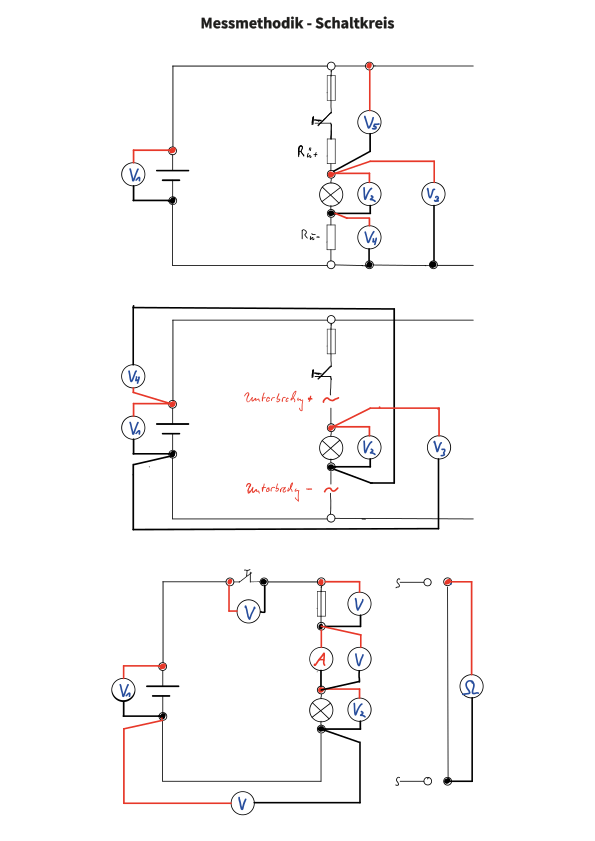
\includegraphics[width=.80\textwidth]{images/Messmethodik_Schaltkreis.pdf}%
  \caption{Messmethodik_Schaltkreis}%\label{fig:Messmethodik_Schaltkreis}%% anpassen
\end{figure}

%\newpage

%\chapter{Quellcode-files}
%\input{archiv/Quellcode-files}

%%%%%%%%%%%%%%%%%%%%%%%%%%%%%%%%%%%%%%%%%%%%%%%%%%

% Tabellen/

%\chapter{PDFs}
%% ju 28-5-22 PDFs.tex 

%\section{Messen}\label{sec:Messen}\index{Messen}


% -------
\section{Messmethodik - Schaltkreis}\label{sec:Messmethodik_Schaltkreis}\index{Messmethodik_Schaltkreis}
\includepdf[pages=-]{Tabellen/PDF/Messmethodik-Schaltkreis.pdf}

% -------
\section{Messprotokoll}\label{sec:Messprotokoll}\index{Messprotokoll}
\includepdf[pages=-]{Tabellen/PDF/Messprotokoll.pdf}







%%%%%%%%%%%%%%%%%%%%%%%%%%%%%%%%%%%%%%%%%%%%%%%%%%

% content/beispiele/tex/

%\chapter{Aufbau-der-Arbeit}
%\input{content/beispiele/tex/Aufbau-der-Arbeit}
%\chapter{LaTeX-Beispiel-beamer}
%\input{content/beispiele/tex/LaTeX-Beispiel-beamer}
%\chapter{Latex-install-Ubuntu}
%\input{content/beispiele/tex/Latex-install-Ubuntu}
%\chapter{Mathe-Aufgaben}
%\input{content/beispiele/tex/Mathe-Aufgaben}
%\chapter{Mathe-Latex}
%\input{content/beispiele/tex/Mathe-Latex}
%\chapter{Sprachlich-formale-Aspekte}
%\input{content/beispiele/tex/Sprachlich-formale-Aspekte}
%\chapter{Text-Formatierungen}
%\input{content/beispiele/tex/Text-Formatierungen}
%\chapter{vorlage-abbildungen}
%\input{content/beispiele/tex/vorlage-abbildungen}
%\chapter{vorlage-literaturangabe-kfz}
%\input{content/beispiele/tex/vorlage-literaturangabe-kfz}
%\chapter{vorlage-literaturangabe-sport}
%\input{content/beispiele/tex/vorlage-literaturangabe-sport}
%\chapter{vorlage-literaturangabe}
%\input{content/beispiele/tex/vorlage-literaturangabe}
